\subsection{Block diagram}
\begin{figure}[h!]
    \centering
    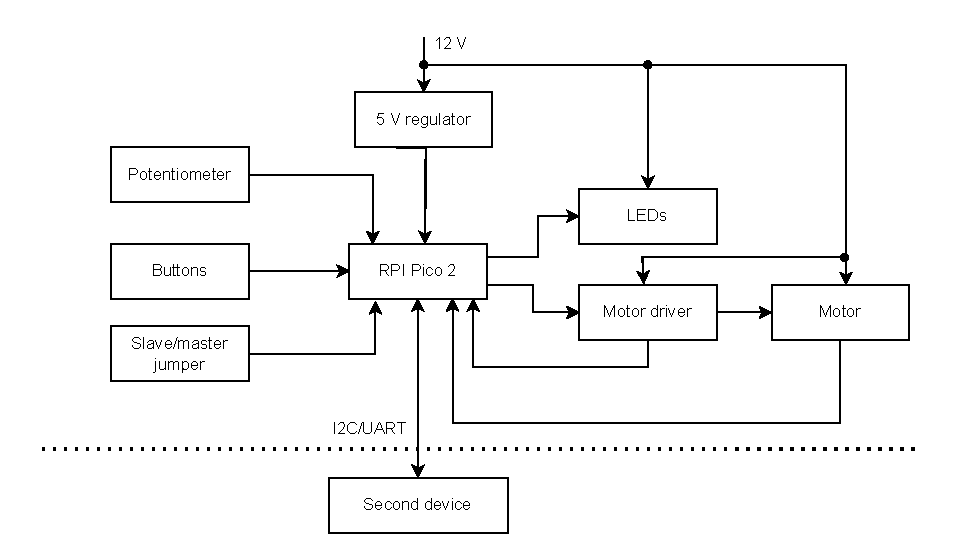
\includegraphics[width=\textwidth]{images/Sideshift-block-diagram.pdf}
    \caption{Block diagram of the treadmill sideshift module.}
    \label{fig:sideshift-block-diagram}
\end{figure}

\subsection{Motor Linak LA14}
Exact model number is Linak 14020130000A0C06:
\begin{itemize}
    \item \textbf{Feedback:} Hall potentiometer
    \item \textbf{Motor type:} 12 V BDC Fast
    \item \textbf{Endstop:} Power switch 
\end{itemize}
The figure \ref{fig:motor_connect} shows the correct connection of the motor to the PCB.
\begin{figure}[h!]
    \centering
    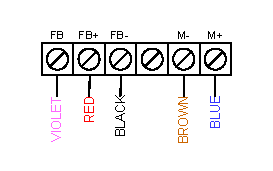
\includegraphics[width=0.5\textwidth]{images/motor_wiring.drawio.pdf}
    \caption{Connecting motor to the PCB.}
    \label{fig:motor_connect}
\end{figure}

\newpage
\subsection{Motor driver DRV8873}
Configuration of the DRV8873 used in this project:

\begin{itemize}
    \item \textbf{Interface:} Hardware
    \item \textbf{Current sensing:} Active over 360 Ohm resistor
    \item \textbf{Control mode:} PH/EN
    \item \textbf{PWM:} Software use 25~kHz
    \item \textbf{Slew rate:} \(13 V/ \mu s \)
    \item \textbf{Current ITRIP regulation:} Enabled
    \item \textbf{Open load diagnostic:} Enabled
\end{itemize}


\begin{figure}[h!]
    \centering
    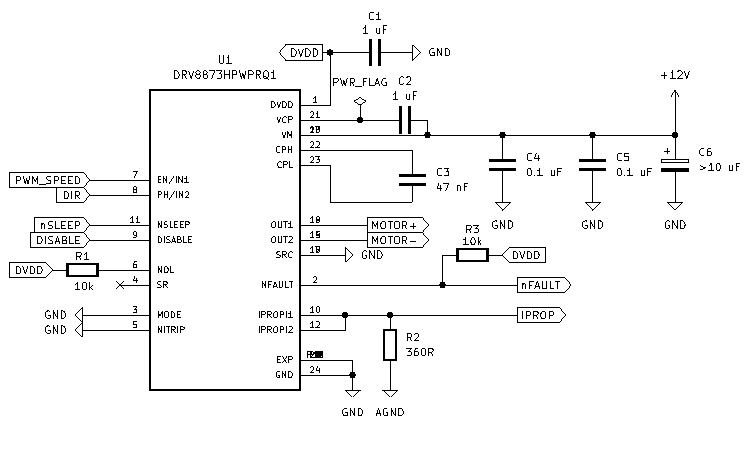
\includegraphics[width=\textwidth]{images/DRV8873H_wiring.pdf}
    \caption{DRV8873H schematic.}
    \label{fig:DRV8873H_wiring}
\end{figure}

\newpage
\subsection{RPi Pico 2}

\begin{figure}[h!]
    \centering
    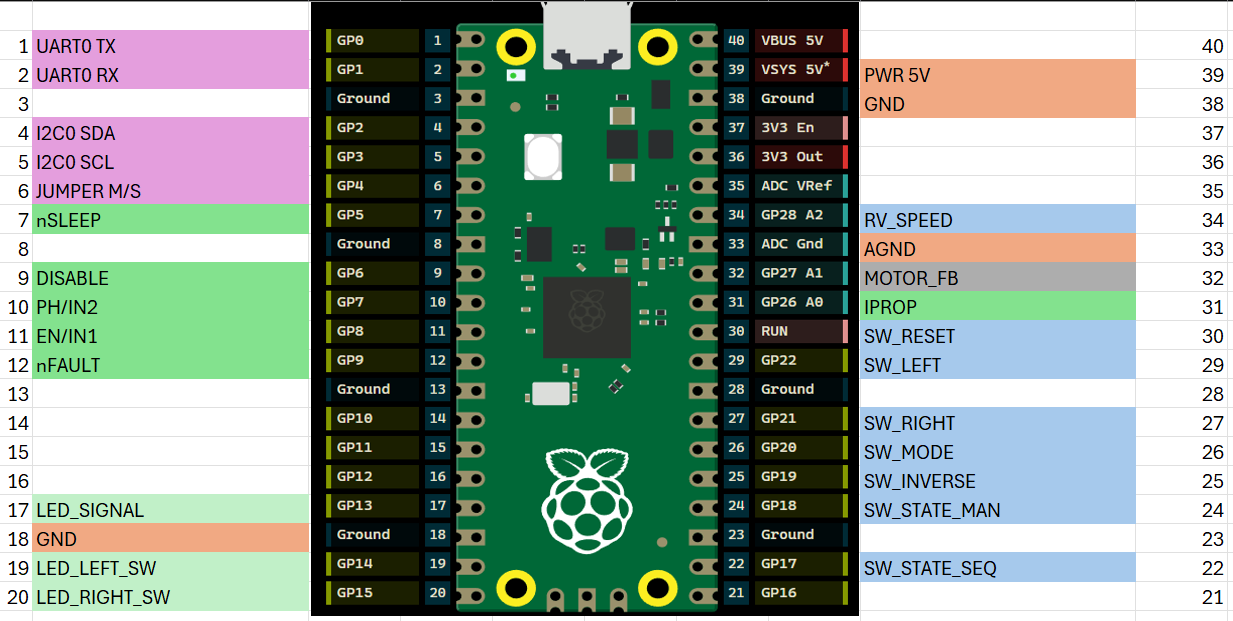
\includegraphics[width=0.9\textwidth]{images/pico_pin_mapping.png}
    \caption{RPi Pico pin mapping.}
    \label{fig:pico_pin_mapping}
\end{figure}

The Raspberry Pi Pico is powered from a 5V regulator and connected through a Schottky diode so that when a USB cable is connected to the Pico, it cannot supply power to the rest of the PCB.

A reset button is placed on the PCB, and when pressed, it grounds the RUN pin, causing the Pico to reset.

\begin{figure}[h!]
    \centering
    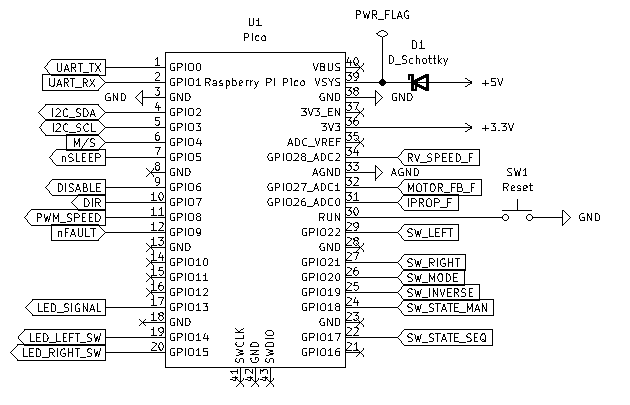
\includegraphics[width=\textwidth]{images/pico_wiring.pdf}
    \caption{RPi Pico schematic}
    \label{fig:pico_wiring}
\end{figure}




\newpage
\subsection{Power supply}
An external 12 VDC power supply is connected to the board, which should be able to provide a current of at least 1.5 to 2 A.


The power input is 12~V is protected by a 5~A fuse based on Table~\ref{tab:power_consumption}, providing protection against reverse polarity and short circuits. In case of reverse polarity, the fuse must be replaced as it will be permanently damaged. As a 5V regulator, the LM7805 is used, and an LED is connected to it to indicate the voltage at the regulator's output. See the schematic in figure \ref{fig:power_schematic}.



\begin{table}[h!]
\centering
\begin{tabular}{|l|c|c|l|}
\hline
\textbf{Component} & \textbf{Supply Voltage (V)} & \textbf{Max Current (mA)} & \textbf{Power Source}\\
\hline
RPI Pico           & 5  & 100  & Regulator (7805) \\
\hline
Driver DRV8833     & 12 & 10   & Power supply \\
\hline
DC motor           & 12 & 2500 & Driver \\
\hline
Motor feedback     & 12 & 1    & Power supply \\
\hline
State LED          & 12 & 20   & Power supply      \\
\hline
Mode button LED    & 12 & 20   & Power supply  \\
\hline
PWR switch LED     & 12 & 20   & Power supply       \\
\hline
\end{tabular}
\caption{Power consumption of individual components}
\label{tab:power_consumption}
\end{table}

\begin{figure}[h!]
    \centering
    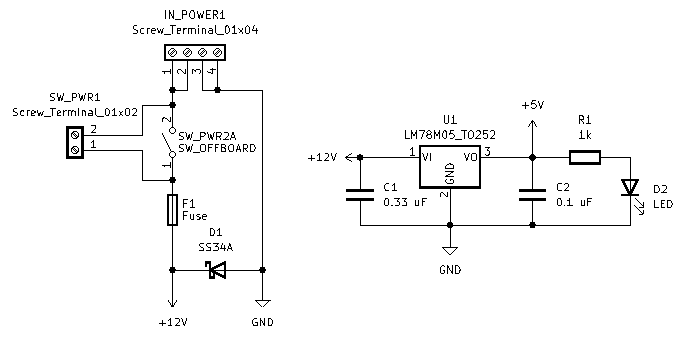
\includegraphics[width=\textwidth]{images/power_schematic.pdf}
    \caption{Power supply schematic.}
    \label{fig:power_schematic}
\end{figure}

\newpage
\subsection{Analog circuits}
All analog signals use simple RC low-pass filters, and their cutoff frequencies are listed in table \ref{tab:rc_filters}. All analog sections also have a separate ground, AGND.

\begin{table}[h!]
\centering
\begin{tabular}{|c|c|c|c|}
\hline
\textbf{Signal} & \textbf{R} & \textbf{C} & \textbf{Cutoff frequency} \\ \hline
Motor feedback & 10 k$\Omega$ & 1 $\mu$F & 15.9 Hz \\ \hline
Potentiometer & 10 k$\Omega$ & 1 $\mu$F & 15.9 Hz\\ \hline
Motor current & 10 k$\Omega$ & 3.3 nF & 4823 Hz\\ \hline
\end{tabular}
\caption{RC Low-pass filters for analog signals}
\label{tab:rc_filters}
\end{table}

\subsubsection{Motor current IPROP}
The motor current is measured using the IPROPI1 and IPROPI2 pins, which are connected together for the purpose of this application. For converting the current into a voltage, the resistor $R_{\text{sense}}$ is used, and its value is determined from the following equation:

 \begin{equation}
	\label{r_sense}
    R_{sense}= \frac{k\cdot U_{max}}{I_0}=\frac{1100 \cdot 3.3}{10} \doteq 360 \; \Omega
\end{equation}

\subsubsection{Motor feedback}
The motor feedback from the LINAK LA14 ranges from 0 to 10\,V; a voltage divider is used to scale it down to 0–3.3\,V for the Raspberry Pi Pico's ADC. In addition, a safety margin is provided so that in the event of a fault, where a voltage of up to 12\,V may appear on the pin, the ADC will not be damaged.
\begin{table}[h!]
\centering
\begin{tabular}{|c|c|c|c|}
\hline
{$U_{in} [V]$} & {$R_1$ [$\Omega$]} & {$R_2$ [$\Omega$]} & {$U_{out} [V]$} \\ \hline
12 & 100k & 36k & 3.18 \\ \hline
\end{tabular}
\caption{Voltage divider for motor feedback input.}
\label{tab:voltage_divider}
\end{table}

\subsection{LEDs}
For panel mounting, the LEDs need to be powered from 12\,V. Therefore, the ULN2004A integrated circuit was used. To set the LED current to approximately 20\,mA, a series resistor of 470\,$\Omega$ was chosen.The LED lights up when a logic high (1) is applied to the corresponding Raspberry Pi Pico pin.

\begin{figure}[h!]
    \centering
    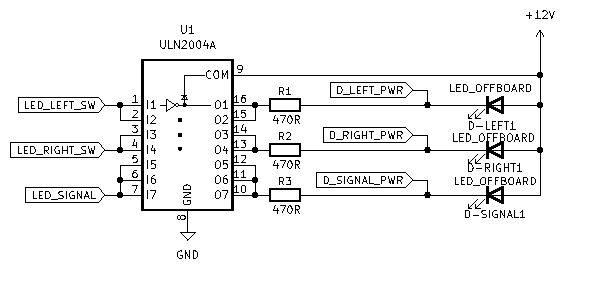
\includegraphics[width=\textwidth]{images/leds_wiring.pdf}
    \caption{LEDs schematic.}
    \label{fig:leds_schematic}
\end{figure}

\newpage
\subsection{Communication}
Communication with the second board is carried out via I\textsuperscript{2}C or UART. When using the I\textsuperscript{2}C bus, it is necessary to set whether the device acts as a master or a slave by means of a hardware jumper. It is necessary to ensure that one board has the jumper set to the slave position and the other board has the jumper set to the master bus position.


\begin{figure}[h!]
    \centering
    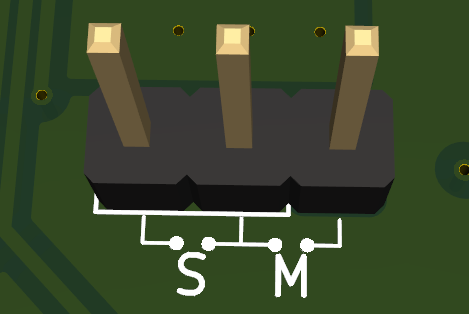
\includegraphics[width=0.2\textwidth]{images/ms_select.png}
    \caption{Master/Slave jumper.}
    \label{fig:ms_select}
\end{figure}

\note{For PCB version v1.0.0, the pin selected for I\textsuperscript{2}C is incorrect, and it is not possible to operate it on the prepared pins. As a temporary solution, the I\textsuperscript{2}C protocol can be used on the UART pins, where Tx corresponds to SDA and Rx corresponds to SCL. Therefore, when switching protocols, it is always necessary to swap the wires.}

\note{
\begin{figure}[h!]
    \centering
    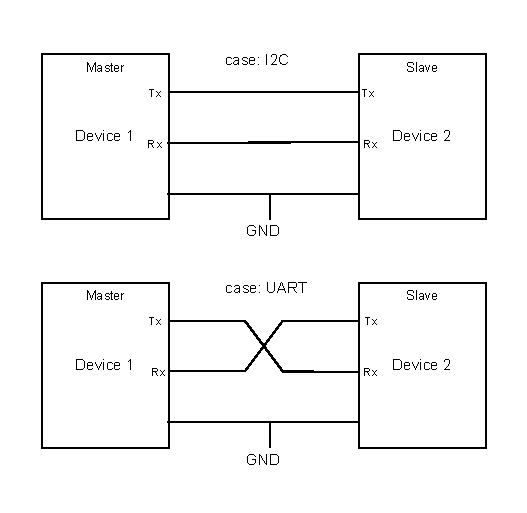
\includegraphics[width=0.63\textwidth]{images/sideshift_master_slave.pdf}
    \caption{\note{Temporary communication wiring.}}
    \label{fig:temp_comm_schematic}
\end{figure}
}


